\pdfoutput=1 % Tell arXiv to use pdfLaTeX. Do not remove this line.

\documentclass[11pt]{article}

% Remove the "review" option to generate the final version.
\usepackage{emnlp2021}
\usepackage{times}
\usepackage{xspace}
\usepackage{latexsym}
\usepackage[T1]{fontenc}
\usepackage[utf8]{inputenc}
\usepackage{microtype}
\usepackage{graphicx}
\usepackage{relsize}
\usepackage{tabularx}
\usepackage{booktabs}
\usepackage{amsmath}
\usepackage{amssymb}
\usepackage{subcaption}
\usepackage{float}
\usepackage{csquotes}
\graphicspath{{figures/}}
\newcommand{\ArgKP}{\mbox{ArgKP-2021}\xspace}
\newcommand{\ArgQ}{\mbox{IBM-ArgQ-Rank-30kArgs}\xspace}
\newcommand{\Bert}{\textsc{Bert}\xspace}
\newcommand{\BertBase}{\Bert-Base\xspace}
\newcommand{\BertLarge}{\Bert-Large\xspace}
\newcommand{\Roberta}{\mbox{Ro\textsc{Bert}a}\xspace}
\newcommand{\RobertaBase}{\Roberta-Base\xspace}
\newcommand{\Albert}{\textsc{Albert}\xspace}

% Draft editing helpers. Remove 
%\newcommand{\todocite}{{\smaller\color{red}[CITE]}\xspace}
%\newcommand{\todo}[1]{{\smaller\color{red}[#1]}}

\title{%
  Modern Talking in Key Point Analysis: \\
  Key Point Matching using Pretrained Encoders%
}
\author{%
  Jan Heinrich Reimer \and Thi Kim Hanh Luu \and Max Henze \and Yamen Ajjour \\
  Martin Luther University Halle-Wittenberg, Germany \\ 
  \texttt{\{%
  \href{mailto:jan.reimer@student.uni-halle.de}{\textcolor{black}{jan.reimer}},%
  \href{mailto:thi.luu@student.uni-halle.de}{\textcolor{black}{thi.luu}},%
  \href{mailto:max.henze@student.uni-halle.de}{\textcolor{black}{max.henze}}%
  \}@student.uni-halle.de} \\ 
  \texttt{\href{mailto:yamen.ajjour@informatik.uni-halle.de}{\textcolor{black}{yamen.ajjour@informatik.uni-halle.de}}}%
}

\begin{document}

\maketitle

\begin{abstract}
  We contribute to the ArgMining~2021 shared task on Quantitative Summarization and Key Point Analysis with two approaches for argument key point matching. 
For key point matching the task is to decide if a short key point matches the content of an argument with the same topic and stance towards the topic. 
We approach this task in two ways: 
First, we develop a simple rule-based baseline matcher by computing token overlap after removing stop words, stemming, 
and adding synonyms/antonyms.
Second, we fine-tune pretrained \Bert and \Roberta language models as a regression classifier for only a single epoch. 
We manually examine errors of our proposed matcher models and find that long arguments are harder to classify. Our fine-tuned \RobertaBase model achieves a mean average precision score of~0.913, the best score for strict labels of all participating teams. 

\end{abstract}

\section{Introduction}\label{introduction}

Arguments influence our decisions in many places of our daily life~\cite{Bar-HaimEFKLS2020}. 
But with the increasingly larger amount of information found on the Web\footnote{\url{https://internetlivestats.com/}} 
and more effective argument mining, people often need to summarize arguments~\cite{LawrenceR2019,Bar-HaimEFKLS2020}. 
\citet{Bar-HaimEFKLS2020} see matching key points to arguments as an intermediate step towards automatically generating 
argumentative summaries~(Section~\ref{related-work}). 
The ArgMining~2021 shared task on Quantitative Summarization and Key Point Analysis~\cite{kpa-2021-overview} is the first task on key point matching, 
which is an important step towards summarizing arguments. 
By matching arguments with a pre-defined set of key points, an argumentative text can be summarized using the prevalence of the key points in it. 
Different approaches of matching argument key point pairs, here called matchers, should be proposed and discussed. 
Given an argument and a key point, a matcher should return a real value between~0 and~1 which represents the extent to which the argument matches the key point.\footnote{\url{https://2021.argmining.org/shared_task_ibm.html}} 
%\todo{Cite the task overview paper once the citation is announced.}
For evaluating different argument key point matchers, the shared task organizers uses mean average 
precision evaluation as a metric~\cite{kpa-2021-overview} to evaluate the approaches and publish the \ArgKP benchmark dataset~(Section~\ref{data}) to compare 
matchers~\cite{Bar-HaimEFKLS2020}. % \todo{Overview paper}

Pretrained language models like \Bert and \Roberta are nowadays becoming standard approaches to tackle various Natural 
Language Processing tasks~\cite{DevlinCLT2019,LiuOGDJCLLZS2019}. 
Because of their extensive pretraining, often fine-tuning these language models with even a small task-specific dataset 
can achieve state-of-the-art performance~\cite{DevlinCLT2019}. 
As the \ArgKP dataset~\cite{Bar-HaimEFKLS2020} used in the ArgMining~2021 shared task on Quantitative Summarization is 
relatively small~(24\,083 labelled pairs), we decide to fine-tune \Bert and \Roberta language models rather than train 
a neural classifier from scratch~(Section~\ref{approach}).

Contrasting this neural approach, we introduce a simple rule-based baseline matcher that compares preprocessed tokens of 
each argument to the tokens of each key point~(Section~\ref{approach}). 
For the baseline, we compute token overlap after removing stop words, adding synonyms and antonyms, and stemming the 
tokens from both argument and key point using the NLTK~toolkit~\cite{BirdL2004}.

Our fine-tuned \RobertaBase matcher achieves a mean average precision score of up to~0.967 and ranks second in the 
shared task's leaderboard~(Section~\ref{results}).
In a manual error analysis, we find that the imbalanced \ArgKP dataset causes neural models to predict non-matching 
argument key point pairs more precisely than matching pairs~(Section~\ref{error-analysis}).
We further observe a tendency that large length differences between arguments and key points can cause errors. 
To encourage researchers to train more robust argument key point matchers, we release our source code under a free license.%
% \footnote{\url{https://github.com/heinrichreimer/modern-talking}}
\section{Related Work}\label{related-work}

% \todo{Shorten subsections. We probably don't need subsection headers in this section.}

% \subsection{Key Point Analysis}



Similar tasks to key point analysis include clustering arguments~\cite{reimers2019classification,ajjour2019modeling}, detecting similar arguments in a pairwise fashion~\cite{misra:2016} and matching arguments to generic-arguments~\cite{naderi:2017}. Using points to summarize arguments were approached by~\citet{egan2016summarising} on online discussion. Points were extracted by using the verbs and their syntactic arguments and are then clustered together to deliver a summary of the discussion. 

Key point analysis is the task of matching a given argument with one or more pre-defined key points~\cite{Bar-HaimEFKLS2020}. To develop models for the task, \citet{Bar-HaimEFKLS2020} introduced a dataset (\ArgKP) which contains 24 093~argument key point pairs on 28~topics. Each argument and key point is labeled manually as \texttt{match} or \texttt{no-match}. The authors experimented with several unsupervised and supervised approaches to perform the task in a cross-topic experimental setting. \Bert~\cite{DevlinCLT2019} performed the best in their experiments by reaching an F1 score of $0.68$.

In a later work, \citet{Bar-HaimKEFLS2020} develop a summarization approach for online discussions that
uses key point analysis. The summrization approach takes as input a set of comments on a given topic and extracts a set of representative key points from them. The output of the summarization approach is the set of extracts key points together with the count of matched comments for each key point. In its essence, the summarization approach uses a matching model that gives a score for a given comment and key point or a pair of key points. For matching models, \citet{Bar-HaimKEFLS2020} compare different variants of  \Bert~\cite{DevlinCLT2019}. Among the tested models, \Albert \cite{lan2019albert} performed the best with an F1 score $0.809$, but \Roberta~\cite{LiuOGDJCLLZS2019} were chosen for key point extraction at the end, which is 6 times faster than \Albert and still achieves an F1 score of $0.773$. 

Our approaches for the key point analysis are based on \Bert and \Roberta. \Bert stands for Bidirectional Encoder Representations from Transformers and is an open-source bidirectional language representation model published by Google~\cite{DevlinCLT2019}. \Bert is pre-trained over unlabeled text to learn a language representation and can be fine-tuned on downstream tasks. During pre-training, \Bert is trained on two unsupervised tasks: Masked Language Model and Next Structure Prediction. \Roberta is an improved variant of \Bert that is introduced by Facebook in 2019~\cite{LiuOGDJCLLZS2019}. \citet{LiuOGDJCLLZS2019} modified \Bert by using a larger training data size of 160GB of uncompressed text, more compute power, larger batch-training size, and optimized hyper-parameters. In comparison to \Bert, pre-training tasks for \Roberta were done with full-length sentences and include only Masked Language Model while applying different masks in each training epoch (dynamic masking). \Roberta outperforms \Bert on all 9 GLUE tasks in the single-task setting and 4 out of 9 tasks in the ensembles setting~\cite{WangSMHLB2018,LiuOGDJCLLZS2019}.



% \subsection{Argument Clustering}
% Argument Clustering is a mighty tool that enables algorithms to assign multiple arguments, which adress a similar
% key message to a given topic. \citet{reimers2019classification} make use of 
% "contextualize word embeddings to classify and cluster topic-dependet arguments". Having performed argument
% classification they then compute similar and dissimilar pairs of arguments. Two approaches one with clustering
% and one without are being used. 
% Clustering arguments is achieved by usage of agglomerative hierarchical clustering \cite{day1984efficient}. 
% Without clustering a fine-tuned BERT-base-uncased model reached a F1 mean score for similar and dissimilar
% arguments of $0.7401$. 
% Agglomerative hierarchical clustering being a strict partitioning algorithm, results for clustering perform
% worse by up to 7.64pp (Bert-large F1 mean score: $0.7135$). Hence they conclude that "strict partitioning 
% clustering methods introduce a new source of errors".
% Another approach proposed by \citet{ajjour2019modeling} revolves around clustering 
% arguments into so called frames which are "a set of arguments that focus on the same aspect". 
% Thereby framing \cite{entman1993framing} only a specific information to present to the listeners and convince 
% them of your stance.
% They propose that an argument consists of two crucial parts. The topic and the frame.
% Hence their approch splits into three steps: First, all arguments are clustered into $m$ topics. Second,
% topical features are extracted from all arguments and therefore from its cluster. Third, the arguments are 
% reclustered into $k$ non-overlapping frames. By utilizing k-means \cite{hartigan1979ak} for clustering
% and Term Frequency-Inverse Document Frequency (TF-IDF) for topic removal they achieved a F1 score of 
% $0.28$.

% \subsection{Pretrained Language Models}




\section{Data}\label{data}
\begin{table*}
    \caption{Examples of argument key point pairs from the \ArgKP dataset~\cite{Bar-HaimEFKLS2020}}
    \label{examples}
    \begin{tabularx}{\linewidth}{lXp{4.3cm}c}
      \toprule
      \textbf{\#} & \textbf{Argument} & \textbf{Key point} \\
      \midrule
      A & % from training set, match
      child \textcolor{violet}{actors} can be overworked and they can miss out on their education. & % arg_13_153
      Being a \textcolor{violet}{performer} harms the child's education \\ % kp_13_5
      B & % from training set, match
      as long as nuclear weapons exist, the entire world has to worry about \textcolor{violet}{nations} deciding to fire them at another or \textcolor{violet}{terrorists} getting hold of them and causing disaster & % arg_17_91	
      Nuclear weapons can fall into the \textcolor{violet}{wrong hands} \\ % kp_17_1
      C & % from training set, not labelled
      `people reach their limit when it comes to their quality of life and should be able to end their \textcolor{violet}{suffering}. this can be done with little or no \textcolor{violet}{suffering} by \textcolor{teal}{assistance} and the person is able to say good bye. & % arg_0_0
      \textcolor{teal}{Assisted} suicide reduces \textcolor{violet}{suffering} \\ % kp_0_1
      \bottomrule
    \end{tabularx}
  \end{table*}

\begin{figure*}
    \centering
    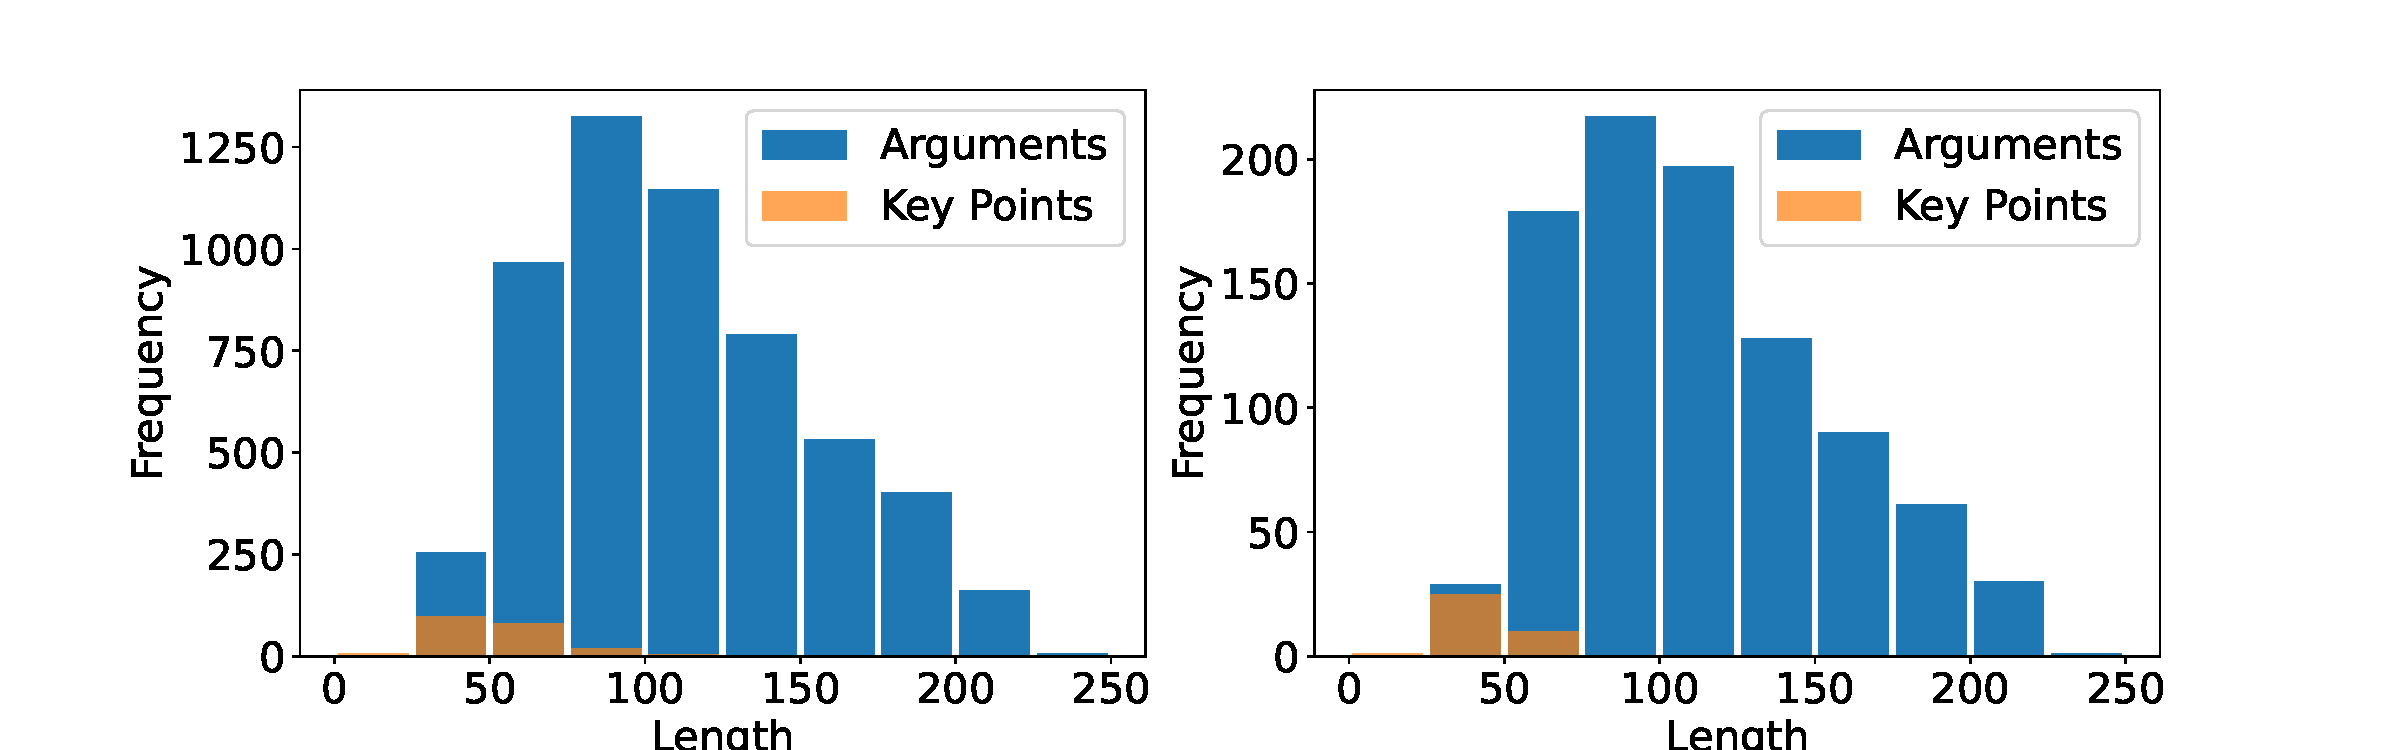
\includegraphics[width=\linewidth]{arg-kp-length.pdf}
    \caption{Lengths in characters for arguments and key points from the training and development set.}
    \label{arg-kp-length}
\end{figure*}

The dataset used in the ArgMining 2021 shared task on Quantitative Summarization and Key Point Analysis is the \ArgKP dataset~\cite{Bar-HaimEFKLS2020} which consists of 24\,083 argument 
and key point pairs labeled as matching/non-matching. They all belong to one of 28~controversial topics, for example: 
\textquote{Assisted suicide should be a criminal offence}. Every key point and argument pair is annotated with its stance towards the topic. 

The training split of the \ArgKP dataset has 5\,583~arguments belonging to 207~key points within 24~topics. This leaves the validation split with 932~arguments and 36~key points for 4~topics.
\citet{kpa-2021-overview} complement the \ArgKP dataset's training and validation split with a test split that is used to evaluate submissions to the shared task. The test split contains 723~arguments with 33~key points from 3~topics.

\subsection{Characteristics}

Here, we do qualitative and quantative analyses of the \ArgKP dataset. Table~\ref{examples} shows examples of argument key point pairs from the \ArgKP dataset~\cite{Bar-HaimEFKLS2020}. 
In pair~A from Table~\ref{examples}, the argument matches the given key point. Both sentences discuss 
children actors and their education. The word \textquote{actors} is not explicitly used in the key point but is 
semantically similar to the word \textquote{performer}. 
Such lexical variation can be opposed by using WordNet~\cite{Miller1995} to find synonyms and antonyms.

Pair~B in Table~\ref{examples} is a harder example, since the argument matches the key point but are expressed differently. 
The key point makes usage of \textquote{wrong hands} as figurative meaning for \textquote{nations} and \textquote{terrorists} from the argument. 
In comparison to pair~A, the linguistic variation in pair~B goes beyond finding synonyms and requires a deep understanding of the semantics of the argument and key point.

Figure~\ref{arg-kp-length} shows the average length of the arguments and key points in the training and developments splits. As shown, the arguments in the \ArgKP dataset are substantially longer than key points.
In the training set, the average length of arguments is 109~characters. 
Compared to that, key points are on average only half as long (52~characters). 
In the validation set, the key points have an average length of 41~characters and therefore key points are shorter than those in the training set. 
The average length of arguments remains almost the same at 108~characters. 
%The differences in length between arguments and key points from the training set and validation set are~57.8 characters and~66.3 characters respectively. 
The proportion of arguments that are 67~characters longer than key points constitute 39\,\%~of the training set 
and 44\,\% of the validation set. 
We can see that there are more short key points in the validation set. 
This length difference might be a challenge for the models in key point matching~(Section~\ref{error-analysis}). Pair~C is an example of an argument and key point pair with a large length difference.

All in all, we identify the following major difficulties in matching key points to arguments: semantically similar words, meaning understanding, and the length difference between the arguments and key points. In the following section, we approach the first two problems while developing our baseline and approaches. In Section~\ref{error-analysis}, we analyze the errors made by our approaches with regard to the length difference between the arguments and key points.
\section{Approach}\label{approach}

To match key points to arguments, we propose two different approaches.
First, we discuss a simple yet effective baseline measuring token overlap between key points and arguments.
Second, to improve upon this simple baseline, we introduce an approach based on \Bert and \Roberta~\cite{DevlinCLT2019,LiuOGDJCLLZS2019}. 
We fine-tune both language models in standard configuration with only minor changes highlighted below.

\subsection{Token Overlap Baseline}
To be able to compare more sophisticated matchers, we first propose a very simple token overlap baseline using preprocessed tokens 
from each argument and key point, as parsed by the NLTK toolkit~\cite{BirdL2004}. 
In general, key points summarize ideas of their matched arguments.
Our intuition, therefore, is that certain words or tokens from an argument are also likely to be present in its matched key points. 
Rather than using completely new words for summarization of arguments, a human would tend to reuse important words from the argument.
% \todo{Do they really? Maybe cite a source. - Tried but didn't find a proportion of abstractive vs. extractive summarazition by humans.}
For example, in the argument and key point pair~C from Table~\ref{examples} both, the argument and key point, contain the token \textquote{suffering}.

We can further increase the token overlap between arguments and key points by preprocessing their tokens as following:
First, we remove stop words for reducing noise within all arguments.
Initially, this can seem counterproductive because with fewer words the highest possible overlap would also decrease and 
therefore could lead to worse performance.
However, a lot of arguments and key points contain functional words like \textquote{the}, \textquote{and} or \textquote{as}.
Removing these results in sentences that contain more specific information and thus leads to less confusion with the token overlap matcher.
%Furthermore, the redundancy of language makes it possible to contain key aspects in sentences, even without these mostly meaningless stop words.
As a second preprocessing step, we reduce tokens to their corresponding stems by applying stemming using the Snowball stemmer~\cite{Porter1980}. 
We expect the token overlap matcher to be able to generalize more when comparing tokens.
For example, the words \textquote{assistance} and \textquote{assisted} from the above example~(Table~\ref{examples},~C) 
are both stemmed to \textquote{assist} with the Snowball stemmer. 
Consequently, stemming creates an overlap between different forms of the same word and, for instance, increases the 
probability that an argument containing \textquote{assistance} is associated with a key point containing \textquote{assisted}.
Last, we increase generalization for token overlap even further by supplementing the set of tokens with synonyms and antonyms~\cite{Miller1995}. 
This step should also increase the chance of overlapping tokens.

To compute the similarity between an argument and a key point, let~\(\text{tokens}_a\) be the set of preprocessed tokens from an 
argument~\(a\) and \(\text{tokens}_k\)~the set of tokens from a key point~\(k\).
We calculate the set of overlapping tokens like this:
\begin{equation}
    \text{overlap}_{a,k} = \{ t : t \in \text{tokens}_a \land t \in \text{tokens}_k \}
\end{equation}
The token overlap matcher returns matching scores based on the overlap size weighted against the minimum size of either 
the argument or the key point:
\begin{equation}
    \text{score}_{a,k} = \frac{ |\text{overlap}_{a,k}| }{ \min\{ |\text{tokens}_a|, |\text{tokens}_k| \} }
\end{equation}
That is, pairs with a higher proportion of tokens that appear both in the argument as well as in the key point are 
classified with a higher matching score.

\subsection{Transformers Fine-tuning}

To improve upon this simple token overlap baseline, we fine-tune \Bert and \Roberta Transformer models for classifying 
argument key point matches~\cite{DevlinCLT2019,LiuOGDJCLLZS2019}.
While \Bert is pretrained on a very large document corpus~(16GB of raw data), \Roberta is pretrained on an even larger corpus~(160GB).
Thus \Roberta models can be fine-tuned on higher end task performance~\cite{LiuOGDJCLLZS2019}.
We tokenize both the arguments and the key points with \Bert's default WordPiece tokenizer and the resulting sequences 
are trimmed to 512~tokens for both models.
We then fine-tune the \BertBase and \RobertaBase variants in the standard sentence-pair regression setting using 
the Simple Transformers library.\footnote{\url{https://simpletransformers.ai/}}
The input to the models is formatted as \texttt{[CLS] argument [SEP] key point [SEP]} for \Bert and \texttt{<s> argument </s></s> key point </s>} for \Roberta respectively.
%\texttt{argument [cls] keypoint}.
For classification, we interpret the regression output value as the probability of an argument matching a key point.
That is, the training labels are always 0~or~1, depending on whether the corresponding pair in the training set matches or not.
Both model variants contain 12~hidden layers with a hidden size of~768 and 12~attention heads.
We train each of the two models for one single epoch at a learning rate of~\( \eta = 2 \cdot 10^{-5} \).
We use an AdamW optimizer with~\( \beta = (0.9, 0.999) \) and zero weight decay~\cite{LoshchilovH2019}.
The optimizer is warmed up with a ratio of~6\,\% of the training data, and we fine-tune both models with the binary cross-entropy loss.
We explore three ways of handling argument key point pairs in the training set with missing ground-truth label. In the first way, we remove those pairs completely from the traning dataset. In the second and third ways, we assume all the arguments and key points with missing labels to be either a \texttt{match} or \texttt{no-match}. By comparing the effectiveness of the models, we find that the first way lead to the best effectiveness on the validation set.
Similarly, we experiment with textual data augmentation\footnote{\url{https://github.com/makcedward/nlpaug}}~(swapping synonyms, 
randomly omitting words) to increase the amount of training data, leading to no improvement on validation scores either.
Thus, for the submitted model, we consider only training pairs that have an associated ground-truth label and do not oversample.
We don't restrict the models output to the interval~\([0,1]\)---like we did for the baseline---, as the shared task did not 
mention constraints on the score value that should be returned by a matcher.

\section{Results}\label{results}
\begin{table*}
  \centering
  \caption{Performance of the random and token overlap baseline, \BertBase, and \RobertaBase models with respect to mean average precision~(mAP), precision~(P), and recall~(R) of the match label. Precision and recall are calculated by deriving boolean labels from the matching scores with a threshold of~0.5 for all approaches. We report scores for the training, validation, and test set in the strict and relaxed label settings, as well as the averages of the two settings. The best result per set is highlighted \textbf{bold}.}
  \label{table-results}
  \smaller
  \setlength{\tabcolsep}{2.5mm}
  \begin{tabularx}{\linewidth}{X>{\hspace{1.0em}}ccc<{\hspace{1.0em}}>{\hspace{1.0em}}ccc<{\hspace{1.0em}}>{\hspace{1.0em}}ccc}
    \toprule
    \textbf{Approach} & 
    \multicolumn{3}{>{\hspace{1.0em}}c<{\hspace{1.0em}}}{\textbf{Strict}} & 
    \multicolumn{3}{>{\hspace{1.0em}}c<{\hspace{1.0em}}}{\textbf{Relaxed}} & 
    \multicolumn{3}{>{\hspace{1.0em}}c}{\textbf{Average}} \\
    \cmidrule(l{1em}r{1em}){2-4} \cmidrule(l{1em}r{1em}){5-7} \cmidrule(l{1em}){8-10}
    & mAP & P & R & 
    mAP & P & R & 
    mAP & P & R \\
    \midrule
    \multicolumn{10}{X}{\emph{Training set}} \\
    \midrule
    Random & 
    0.260 & 0.173 & 0.500 & 
    0.409 & 0.330 & 0.501 & 
    0.335 & 0.252 & 0.501 \\
    Token Overlap & 
    0.541 & 0.269 & 0.323 & 
    0.653 & 0.435 & 0.275 & 
    0.597 & 0.352 & 0.299 \\
    \BertBase & 
    0.889 & \textbf{0.703} & \textbf{0.864} & 
    \textbf{0.981} & \textbf{0.936} & \textbf{0.607} & 
    0.935 & \textbf{0.819} & \textbf{0.736} \\
    \RobertaBase & 
    \textbf{0.915} & 0.702 & 0.820 & 
    0.979 & 0.927 & 0.572 & 
    \textbf{0.947} & 0.814 & 0.696 \\
    \midrule
    \multicolumn{10}{X}{\emph{Validation set}} \\
    \midrule
    Random & 
    0.232 & 0.180 & 0.523 & 
    0.430 & 0.364 & 0.524 & 
    0.331 & 0.272 & 0.524 \\
    Token Overlap & 
    0.643 & 0.219 & 0.390 & 
    0.802 & 0.416 & 0.366 & 
    0.722 & 0.317 & 0.378 \\
    \BertBase & 
    0.717 & 0.397 & \textbf{0.802} & 
    0.928 & 0.648 & \textbf{0.649} & 
    0.822 & 0.522 & \textbf{0.725} \\
    \RobertaBase & 
    \textbf{0.879} & \textbf{0.567} & 0.799 & 
    \textbf{0.984} & \textbf{0.816} & 0.569 & 
    \textbf{0.932} & \textbf{0.692} & 0.684 \\
    \midrule
    \multicolumn{10}{X}{\emph{Test set}} \\
    \midrule
    Random & 
    0.237 & 0.150 & 0.545 & 
    0.355 & 0.286 & 0.549 & 
    0.296 & 0.218 & 0.547 \\
    Token Overlap & 
    0.483 & 0.232 & 0.225 & 
    0.575 & 0.350 & 0.178 & 
    0.529 & 0.291 & 0.201 \\
    \BertBase & 
    0.827 & 0.326 & \textbf{0.848} & 
    0.940 & 0.526 & \textbf{0.721} & 
    0.883 & 0.426 & \textbf{0.784} \\
    \RobertaBase & 
    \textbf{0.913} & \textbf{0.490} & 0.741 & 
    \textbf{0.967} & \textbf{0.716} & 0.569 & 
    \textbf{0.940} & \textbf{0.603} & 0.655 \\
    \bottomrule
  \end{tabularx}
\end{table*}


Submissions to the ArgMining~2021 shared task on Quantitative Summarization and Key Point Analysis are evaluated with 
respect to mean average precision~\cite{kpa-2021-overview}. 
%\footnote{\url{https://2021.argmining.org/shared_task_ibm.html}}
%\todo{Overview paper.}
The organizers calculate the score by pairing each argument with the best matching key point according to the predicted 
matching probabilities. 
Within each topic-stance combination, only 50\,\% of the arguments with the highest predicted matching score are then 
considered for evaluation. 
The task organizers claim that this removal of 50\,\% of the pairs is necessary because some arguments do not match any 
of the key points, which would influence mean average precision negatively~\cite{kpa-2021-overview}. 
For the remaining argument key point pairs in each topic-stance combination, the average precision is calculated and the 
final score is computed as the mean of all average precision scores.

The task organizers consider two evaluation settings: strict and relaxed.
Both settings are based on the ground-truth labels from the \ArgKP dataset~\cite{Bar-HaimEFKLS2020}. The two evaluation settings are created to account for argument key point pairs in the \ArgKP with undecided labels~(i.e. not enough agreement between annotators). In the strict setting,
the shared task organizers consider those undecided pairs as \texttt{no-match}. In the relaxed setting, however, the shared task organizers consider the undecided pairs as \texttt{match}~\cite{kpa-2021-overview}. % \todo{Overview paper.}
The mean average precision score is then calculated in the two settings based on the ground-truth labels and the derived labels for the undecided pairs. 
We stress that in this complex evaluation setup, the mean average precision score in the relaxed setting would 
favor assuming matches in case of model uncertainty. 
In comparison, in the strict setting mean average precision would favor assuming \texttt{no-match} between an argument and key point.
However, we find that because only the most probable matching key point is being considered for evaluation, this effect is minor.
The evaluation score in general favors matchers that can match a single key point for each argument with high precision.
It is however not important if a matcher does predict non-matches with high certainty.

\subsection{Discussion}
In Table~\ref{table-results}, we report mean average precision in the strict and relaxed settings of the training, 
validation, and test set in the \ArgKP dataset.
We complement the mean average precision scores by adding precision and recall scores of the \texttt{match} label, 
both in the strict and relaxed setting. To calculate precision and recall, we label an argument and key point pair as \texttt{match} if their score is higher than~0.5 and as \texttt{no-match} otherwise.
To aggregate results of the strict and relaxed settings, we also report the average score of the two variants.
The reported scores should allow for automated and unbiased evaluation of our models and easier comparison with competitive approaches.
We report all 27~scores for the token overlap baseline model as well as for the fine-tuned \BertBase and \RobertaBase models.
To make our results more comparable, we add a second baseline, where matches between arguments and key points of same 
topic and stance are predicted with uniform random probability.
That random baseline represents a worst-case matcher and any weak matcher should exceed its evaluation scores.

The token overlap baseline achieves a mean average precision of~0.483 in the strict setting and~0.575 in the relaxed 
setting on the test set.
Thus, it is nearly twice as good as a random matcher with respect to mean average precision.
Even though this baseline has reasonably good scores on all datasets, we are concerned about the large discrepancies 
between its scores on the validation set and the training and test dataset. 
The rather simple baseline captures the similarity between an argument and a key point on the token level and might be sensative against more complicated parphrases.

Both fine-tuned matchers outperform the baselines by a large margin.
While the \BertBase matcher achieves higher relaxed mean average precision on the training set than the \RobertaBase 
matcher, the \RobertaBase matcher is overall better than \Bert, especially with strict labels.
The \RobertaBase matcher achieves a mean average precision of~0.913 in the strict setting on the test set, and~0.967 
in the relaxed setting.
As these scores on the test set are nearly as high as on the training set, we argue that \Roberta is a more robust 
language model and generalizes better than \Bert.
Also the \RobertaBase matcher performs better in terms of precision, while the \BertBase matcher is better with respect to 
recall for all dataset splits in both the strict and relaxed settings.

\section{Error Analysis}\label{error-analysis}
\begin{figure*}
    \centering
    \begin{subfigure}{0.49\linewidth}
        \vspace*{-1ex}
        \centering
        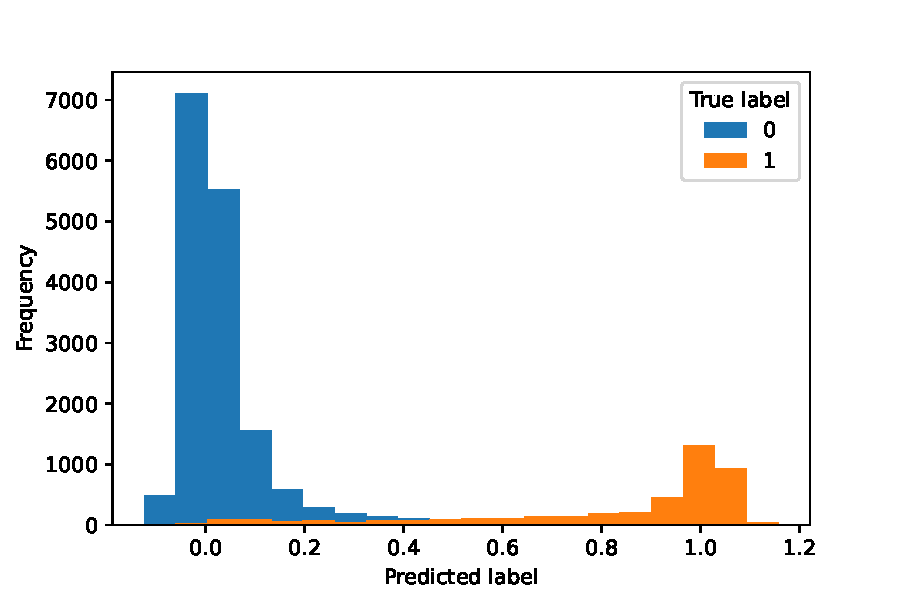
\includegraphics[width=\linewidth]{histogram-labels-bert-train.pdf}
        \vspace*{-3ex}
        \subcaption{Predictions with \BertBase on the training set.}
        \label{subfig:bert_train}
    \end{subfigure}
    \hfill
    \begin{subfigure}{0.49\linewidth}
        \vspace*{-1ex}
        \centering
        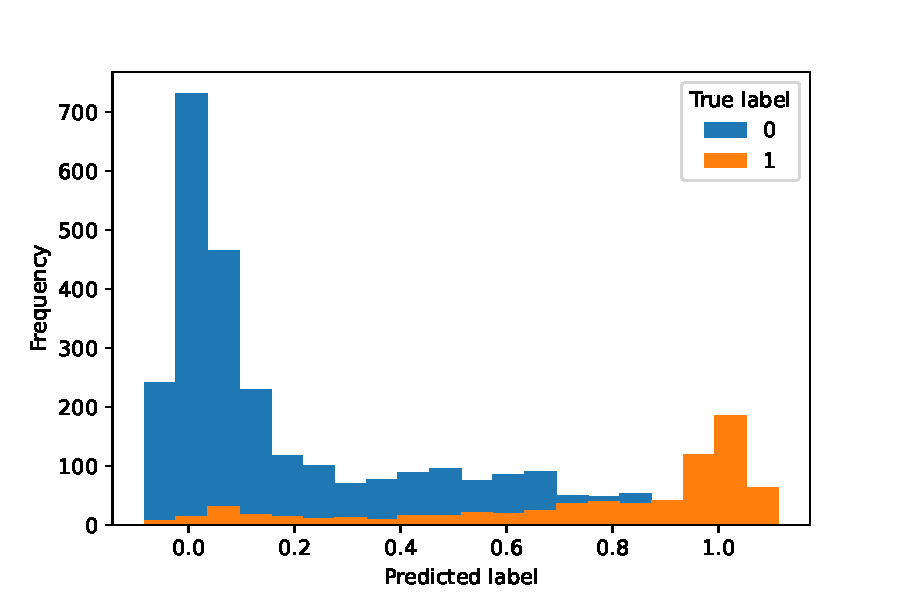
\includegraphics[width=\linewidth]{histogram-labels-bert-dev.pdf}
        \vspace*{-3ex}
        \subcaption{Predictions with \BertBase on the validation set.}
        \label{subfig:bert_dev}
    \end{subfigure}
    \begin{subfigure}{0.49\linewidth}
        \vspace*{-1ex}
        \centering
        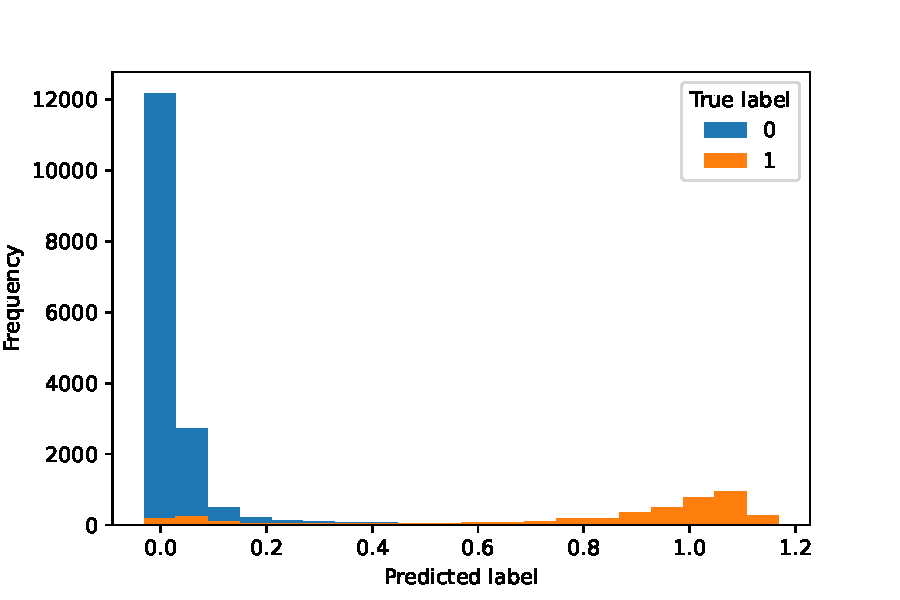
\includegraphics[width=\linewidth]{histogram-labels-roberta-train.pdf}
        \vspace*{-3ex}
        \subcaption{Predictions with \RobertaBase on the training set.}
        \label{subfig:roberta_train}
    \end{subfigure}
    \hfill
    \begin{subfigure}{0.49\linewidth}
        \vspace*{-1ex}
        \centering
        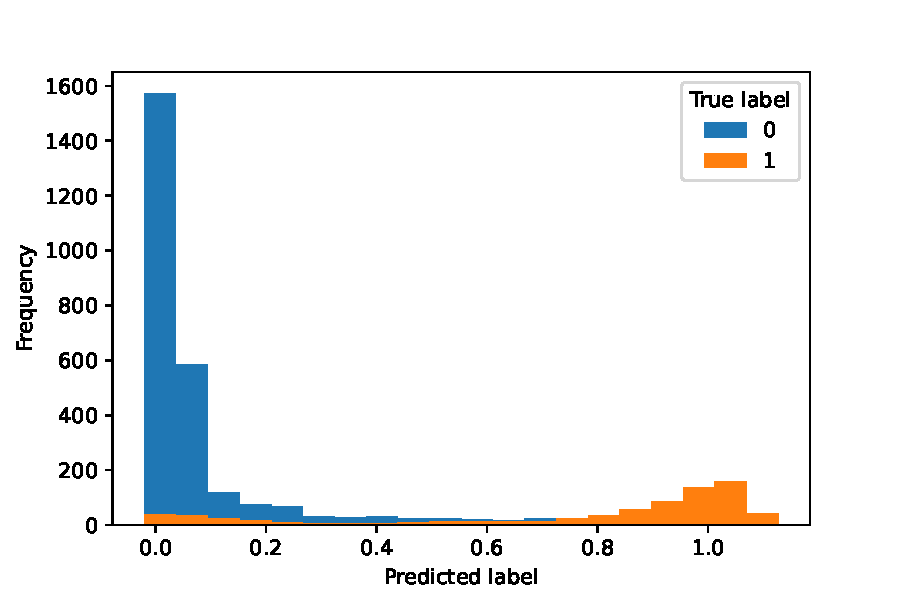
\includegraphics[width=\linewidth]{histogram-labels-roberta-dev.pdf}
        \vspace*{-3ex}
        \subcaption{Predictions with \RobertaBase on the validation set.}
        \label{subfig:roberta_dev}
    \end{subfigure}
    \caption{Histograms of predicted labels on the training and validation sets for argument key point pairs with the \BertBase and \RobertaBase classifiers. For good classifiers, predicted labels should approximately equal the true label~(0~or~1).}
    \label{fig:frequency}
\end{figure*}

\begin{table*}
    \caption{Examples of argument key point pairs from the \ArgKP dataset~\cite{Bar-HaimEFKLS2020} where the predicted score is off the ground truth label~(True) with either the \BertBase or \RobertaBase matcher.}
    \label{error-examples}
    \begin{tabularx}{\linewidth}{lXp{2.5cm}ccc}
      \toprule
      \textbf{\#} & \textbf{Argument} & \textbf{Key point} & \textbf{True} & \textbf{\Bert} & \textbf{\Roberta} \\
      \midrule
      D & % from validation set
      School uniforms can be less comfortable than students' regular clothes. & % arg_4_162
      School uniforms are expensive & % kp_4_6
      0 & \phantom{-}0.48 & 0.03 \\
      E & % from validation set
      affirmative action discriminates the majority, preventing skilled workers from gaining employment over someone less qualified but considered to be a member of a protected minority group. & % arg_15_113
      Affirmative action reduces quality & % kp_15_7
      1 & -0.05 & 0.03 \\
      % F & % from validation set
      % affirmative action can lead to people who are less qualified getting positions they would otherwise not be able to achieve, & % arg_15_110
      % Affirmative action reduces quality & % kp_15_7
      % 1 & -0.04 & 0.01 \\
      \bottomrule
    \end{tabularx}
  \end{table*}
  
%\begin{figure}
    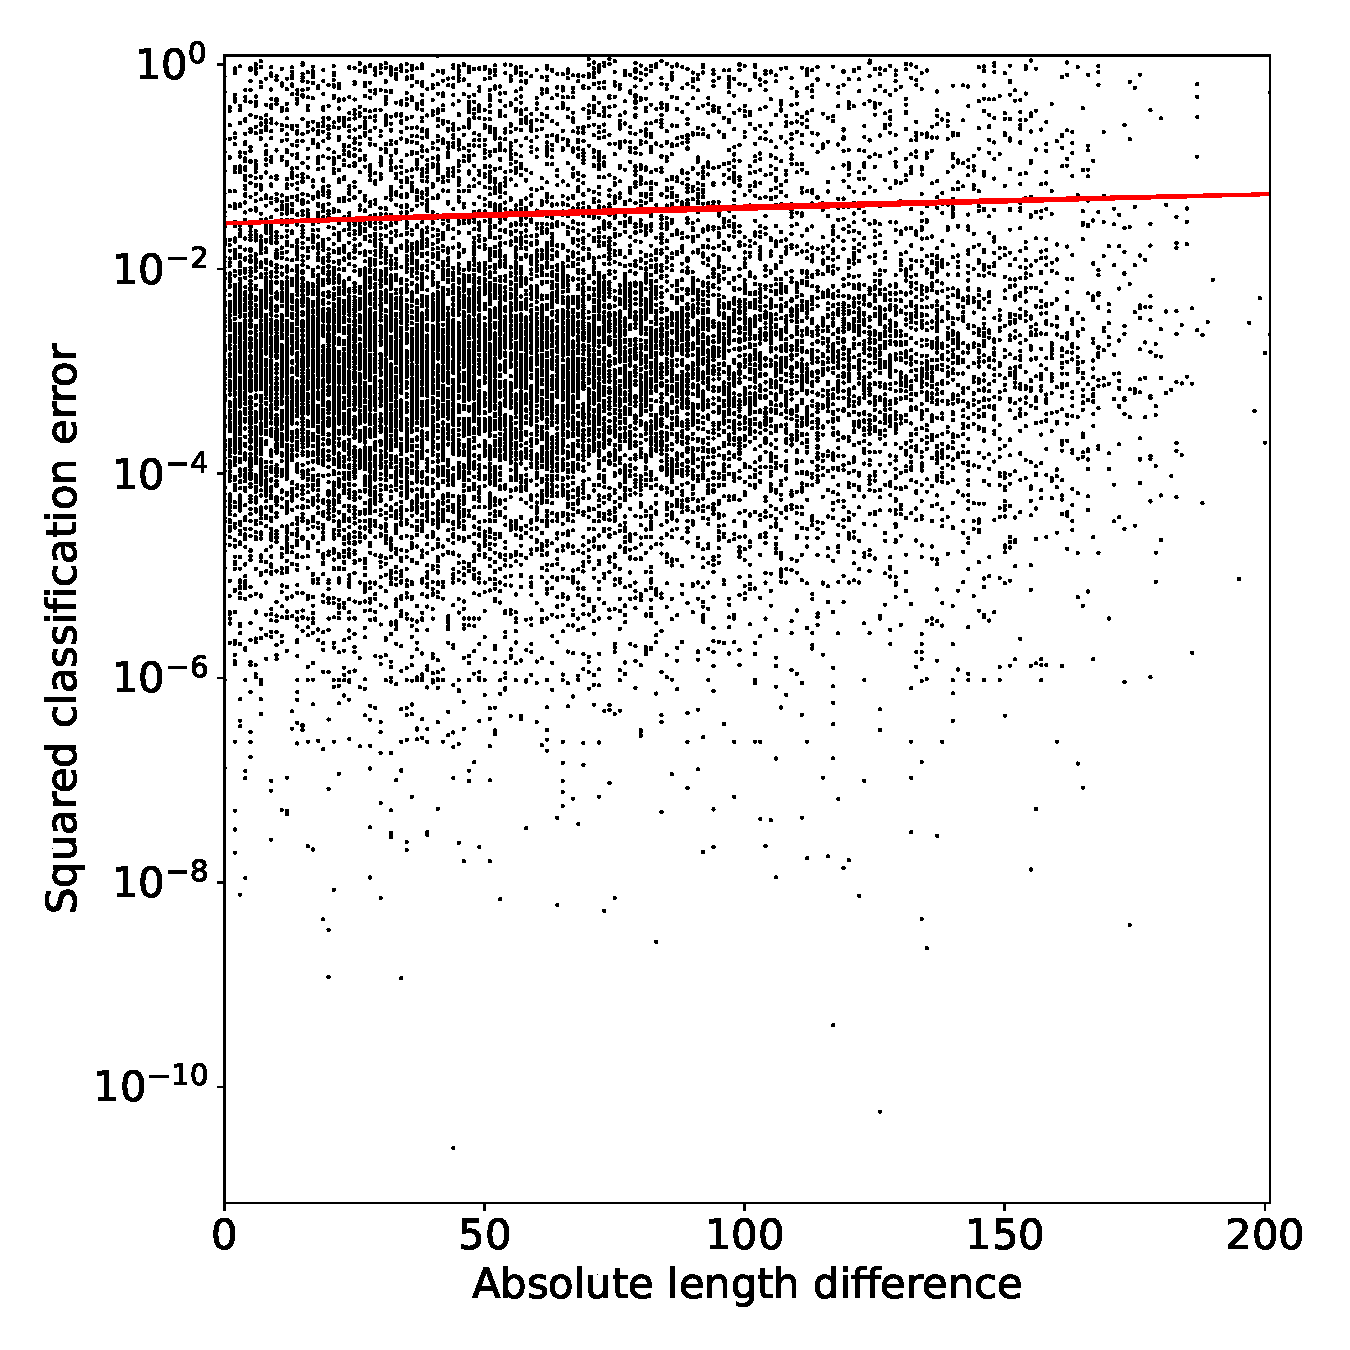
\includegraphics[width=\linewidth]{classification-error-length-difference-bert-train.pdf}
    \vspace*{-5ex}
    \caption{Squared classification error and absolute length difference between in characters each argument and key point pair from the validation set with the \BertBase matcher. The red line indicates the least squares polynomial fit.}
    \label{classification-error-length}
\end{figure}


To find errors of the two trained matchers, \BertBase and \RobertaBase, in Figure~\ref{fig:frequency} we show 
histograms of predicted match scores with respect to ground-truth labels.
Both matchers classify most pairs correctly, which can be seen because the histogram spikes around~0 for the 
true \texttt{no-match} label and around~1 for the true \texttt{match} label.
We also observe that predictions on the training set are closer to the true label than on the development set for both \RobertaBase and \BertBase. 
Even though we expect any machine-learned matcher to perform better on training data than on validation data, 
we see this as a room for improvement with better generalization.
We notice that in Figures~\ref{subfig:bert_train} and~\ref{subfig:roberta_train} both approaches predict non-matching 
argument key point pairs better than matching key points.
This effect is likely to occur because of the higher amount of non-matching pairs provided in the training dataset.
Most arguments match with only a few or even just a single key point.
But nonetheless each argument is compared to all other key points; hence, the underlying data to learn from is 
imbalanced~\cite{BarandelaVSF2004}.
Even though experiments with using textual data augmentation or simple oversampling to balance the dataset were 
unsuccessful~\cite{Dietterich1995}, more advanced oversampling or undersampling approaches could possibly resolve this issue.
We further identify that the predicted matching scores of \BertBase are spread a 
bit more than scores from \RobertaBase.

In Figure~\ref{subfig:bert_dev}, we observe that the \BertBase matcher falsely predicts certain non-matching pairs with scores around~0.5.
An example of such uncertain pair is the argument key point pair~D from Table~\ref{error-examples}.
This argument which is in the training dataset has no matching key points.
For this argument, the \mbox{\BertBase} matcher has not learned well how to classify matches for that type of argument, and therefore predicts a neutral score of~\(0.48\).
However, the \RobertaBase matcher does not make that error. 

Both, the \BertBase matcher and \RobertaBase falsely predict some argument key point pairs as \texttt{no-match} that are in 
fact labelled as a \texttt{match}.
For example, it seems to be difficult to predict a \texttt{match} for the argument key point pair~E from Table~\ref{error-examples}.
The argument from the example is longer than most arguments and especially much longer than the key point~(431\,\%~more characters).
It might be more challenging to reduce such longer arguments, that contain more complex information, to very compact key points.
We confirm that observation by comparing the squared classification error with respect to the absolute difference between 
argument and key point lengths.
%Figure~\ref{classification-error-length} shows a tendency of higher error with the \BertBase matcher when the length difference between the argument and key point is large.
%Comparable results can be observed for the \RobertaBase matcher.
%We therefore identify length difference as a second general problem for both approaches.

\section{Conclusion and Future Work}\label{conclusion}

We approach the practical problem of matching arguments with short key points with the goal of summarizing arguments.
Although our token overlap baseline approach is very simple, it achieves a mean average precision of up to~0.575 on 
the test set, nearly double the score of a random matcher. 
The baseline approach is straightforward to implement but can not eliminate the problem of context understanding. 
\RobertaBase and \BertBase have achieved good performance, because they can overcome the context understanding challenge. 
Our fine-tuned \RobertaBase model also performed better than \BertBase in this task and scores a mean average 
precision of up to~0.967.
With strict ground truth labels it achieves a mean average precision score of~0.913 on the test set, which is the best 
score of the participating teams in the shared task.
This again shows the importance of architecture, training objectives, and hyperparameter selection.

\subsection{Future Work}

In Section~\ref{error-examples}, we observed that transformer models tend to misclassify argument key point pairs if the argument and key point largely differ in length. As an extension to our approach, we propose to combine transformer models with the overlap baseline in an ensemble. Another possible improvement are recent improvements in language models~\cite{Sun2021WFDPSLCZLLWGLSSLOYTWW}.
If a language model is even more robust than, for example, \Roberta, we expect a fine-tuned matcher to outperform the \RobertaBase matcher as well.


% Entries for the entire Anthology, followed by custom entries
\bibliography{anthology,custom}
\bibliographystyle{acl_natbib}

\appendix

% \appendix
% \section{Appendix}

% {\color{red}
%     \subsection{ToDo's}
%     \begin{itemize}
%         \item key-point vs. key point vs. keypoint
%         \item pretrained vs. pre-trained
%         \item comma separator: \verb|.|
%         \item thousands separator: \verb|\,|
%     \end{itemize}
% }


\end{document}
